\documentclass[a4paper, fontsize=14pt]{article}

\usepackage[T2A]{fontenc}
\usepackage[utf8]{inputenc}
\usepackage[russian]{babel}

\usepackage[unicode, pdftex]{hyperref}
\usepackage{lastpage}
\usepackage{float}
\usepackage{gensymb}
\usepackage{booktabs}
\usepackage{amsmath}
\usepackage{amssymb}
\usepackage{tikz}
\usetikzlibrary{shapes, arrows}

\usepackage{graphicx}
\usepackage{subcaption}

\usepackage{geometry}
\geometry{margin=1cm}

\title{Q-learning динамика на графе: постановка, сходимость и сравнение с динамикой Константинова}
\author{}
\date{}

\begin{document}
\maketitle

\section{Введение}
Рассматривается динамика обучения с подкреплением в сетевых социальных дилеммах.
Цель работы --- формализовать модель, описать используемые правила обучения
(Q-learning и SARSA), и сопоставить получаемую динамику кооперации с базовой
динамикой Константинова. Отдельное внимание уделяется ``гранулярному''
монте-карло обновлению, когда за один раунд активна только локальная гранула
узлов, что повышает стохастичность процесса и может поддерживать локальные
кластеры кооператоров.

\section{Формальная постановка модели}
\subsection{Граф и агенты}
Пусть задан неориентированный граф $G=(V,E)$ с $|V|=n$.
Матрица смежности $W=(w_{ij})$ определяет структуру взаимодействий,
а множество соседей агента $i$ обозначим $N_i$.
Каждый агент выбирает стратегию $x_i \in \{0,1\}$
(0 --- Defect, 1 --- Cooperate).
В экспериментах используются графы: звезда, колесо и малый мир
(Watts--Strogatz) с параметрами $N$, $k$ и $p$.

\subsection{Игра и выплаты}
Игра задается типом наград и правилами взаимодействия.
Система поддерживает четыре модели наград:
\begin{align}
\text{pp: } g_i &= b \sum_{j \in N_i} w_{ij} x_j - c \, x_i \, k_i, \\
\text{pf: } g_i &= b \sum_{j \in N_i} w_{ij} x_j - c \, x_i, \\
\text{ff: } g_i &= b \sum_{j \in N_i} \frac{w_{ij} x_j}{k_j} - c \, x_i, \\
\text{fp: } g_i &= b \sum_{j \in N_i} \frac{w_{ij} x_j}{k_j} - c \, x_i \, k_i,
\end{align}
где $k_i$ --- степень узла $i$, $b$ --- выгода, $c$ --- издержки кооперации.

Реализованы три режима игры:
(1) попарная игра на всех ребрах;
(2a) Monte Carlo попарная игра на индуцированном подграфе;
(2b) Monte Carlo игра ``всеми выбранными игроками сразу''.

\subsection{Базовая динамика (по Константинову)}
В качестве базовой точки сравнения используется динамика Константинова.
Основная метрика кооперации:
\begin{equation}
\rho(t) = \frac{1}{n} \sum_{i=1}^n x_i(t).
\end{equation}
В экспериментах теоретические значения $\rho$ для отдельных $b$
используются как ориентиры на графиках.

\section{Q-learning динамика}
\subsection{Определение состояния и Q-функции}
Состояние агента $i$ определяется числом кооперирующих соседей
$s_i = \sum_{j \in N_i} x_j$ на релевантном подграфе.
Q-функция хранится таблично: $Q_i(s,a)$.

\subsection{Политика выбора действий}
Используются две политики выбора действий:
\begin{align}
\text{epsilon-greedy: } & P(a) = \frac{\varepsilon}{|A|} + (1-\varepsilon)\,[a=\arg\max_{a'} Q(s,a')], \\
\text{Boltzmann: } & P(a) \propto \exp\left(\frac{Q(s,a)}{T}\right),
\end{align}
где $T$ --- температура, $\varepsilon$ --- параметр исследования.

\subsection{Правило обновления}
Для Q-learning:
\begin{equation}
Q_i(s_t,a_t) \leftarrow Q_i(s_t,a_t) + \alpha\left[r_{i,t} + \gamma \max_{a'} Q_i(s_{t+1},a') - Q_i(s_t,a_t)\right].
\end{equation}
Для SARSA:
\begin{equation}
Q_i(s_t,a_t) \leftarrow Q_i(s_t,a_t) + \alpha\left[r_{i,t} + \gamma Q_i(s_{t+1},a_{t+1}) - Q_i(s_t,a_t)\right].
\end{equation}

\section{Сходимость}
\subsection{Формулировка результата}
При стандартных условиях на $\alpha_t$ и достаточном исследовании
табличный Q-learning сходится к оптимальным значениям Q-функции
в стационарной среде. В многоагентной среде это условие нарушается,
поэтому результат интерпретируется как эмпирическая динамика
кооперации и поиск устойчивых режимов.

\subsection{Доказательство}
Доказательство опирается на стандартные факты теории стохастической
аппроксимации и классические результаты по сходимости Q-learning
в марковских средах при убывающем шаге обучения.

Сейчас докажем при одновременной игре всех агентов:
$$ Q_i^*(s, a) = \mathbb{E}[R_i(a)] + \gamma \sum_{s'} P(s'|s,a) \max_{a'} Q_i^*(s', a') $$
В пределе $\tau \to \infty$ и при $\gamma < 1$:
$$ Q_i^*(a) \approx R_i(s,a) $$
При больцмановской политике:
$$ P(a) = \frac{e^{Q(s,a)/T}}{\sum_{a'} e^{Q(s,a')/T}} $$
$$ P(a) \approx \sigma(\Delta Q(s,a)/T) $$
В случае награды pp:
$$ \mathbb{E}[R_i(a)] = b \cdot \sum_{j \in N_i} \mathbb{E}[x_j] - c \cdot k_i \cdot a $$
$$ \Delta Q_i^*(s) \approx (b \cdot \sum_{j \in N_i} \mathbb{E}[x_j] - c \cdot k_i \cdot 1) - (b \cdot \sum_{j \in N_i} \mathbb{E}[x_j] - c \cdot k_i \cdot 0) = - c \cdot k_i $$
$$ P(a=1) \approx \sigma(-c \cdot k_i / T) = \frac{1}{1 + e^{c \cdot k_i / T}} $$
$$ \hat{\rho} \approx \frac{1}{n} \sum_{i=1}^n P(a_i=1) = \frac{1}{n} \sum_{i=1}^n \frac{1}{1 + e^{c \cdot k_i / T}} $$

В случае $k_{anchors} = 1$:
$$ \mathbb{E}[R_i(a)] = b \cdot \sum_{j \in N_i} (P(j \ is \ anchor) + \sum_{k} [P(l \ is \ anchor) * \omega_{k_j}]) - c \cdot k_i \cdot a  = $$
$$ = b \cdot \sum_{j \in N_i} \left(\frac{1}{n} + \frac{1}{n} \sum_{l \in N_j} \omega_{l,j}\right) - c \cdot k_i \cdot a $$
$$ \Delta Q_i^*(s) \approx b \cdot \sum_{j \in N_i} \left(\frac{1}{n} + \frac{1}{n} \sum_{l \in N_j} \omega_{l,j}\right) - c \cdot k_i -b \cdot \sum_{j \in N_i} \left(\frac{1}{n} + \frac{1}{n} \sum_{l \in N_j} \omega_{l,j}\right) = - c \cdot k_i$$
А значит опять $$ \hat{\rho} \approx \frac{1}{n} \sum_{i=1}^n P(a_i=1) = \frac{1}{n} \sum_{i=1}^n \frac{1}{1 + e^{c \cdot k_i / T}} $$

\subsection{Обсуждение и сравнение с динамикой Константинова}
Если переходы состояния не зависят от действия агента,
то разность Q-значений сводится к разности мгновенных наград,
и стационарная вероятность кооперации аппроксимируется как
\begin{equation}
p_i \approx \frac{1}{1 + \exp\left(\frac{c k_i}{T}\right)}.
\end{equation}


В многоагентной динамике предпосылка независимости нарушается,
что приводит к наблюдаемой зависимости кооперации от параметра $b$.

\section{Численные эксперименты}
\subsection{Настройки эксперимента}
Используются графы типа звезда и малый мир.
В экспериментах со звездообразным графом: $N=100$, $b \in \{1,\dots,9\}$,
$c=1$, $k_{anchors}=1$, $\alpha=0.2$, $\gamma \approx 0.99$, $T=1.0$,
число эпизодов --- до 15000, число запусков --- до 100.

В экспериментах на малом мире: $N$ от 50 до 100,
$k=4$, $p=0.1$, $b$ фиксируется или варьируется,
$T \in \{0.5, 1.0, 2.0\}$, $c=1.0$,
используется Monte Carlo режим с локальными гранулами.

\subsection{Графики сходимости}
\begin{figure}[H]
	\centering
	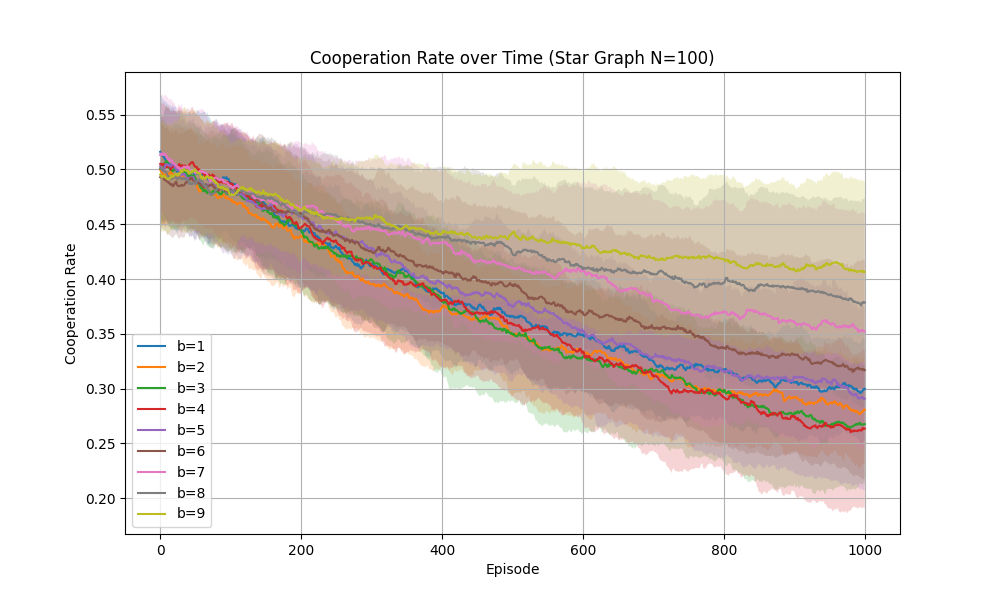
\includegraphics[width=0.9\textwidth]{../results/star_graph_over_time.png}
	\caption{Звезда: динамика кооперации во времени.}
	\label{fig:star_over_time}
\end{figure}

\begin{figure}[H]
	\centering
	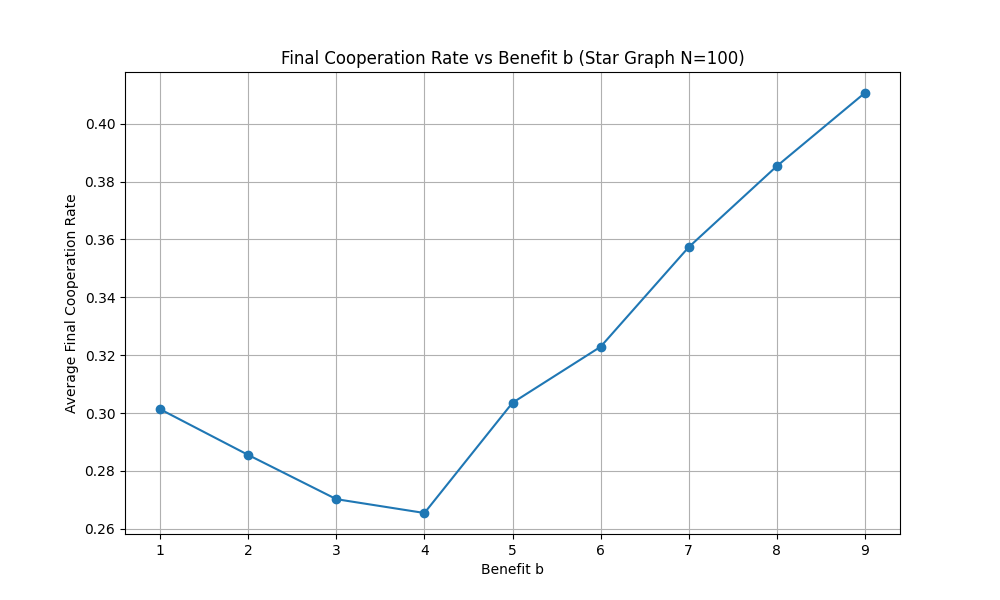
\includegraphics[width=0.8\textwidth]{../results/star_graph_vs_b.png}
	\caption{Звезда: финальная кооперация в зависимости от $b$.}
	\label{fig:star_vs_b}
\end{figure}

\begin{figure}[H]
	\centering
	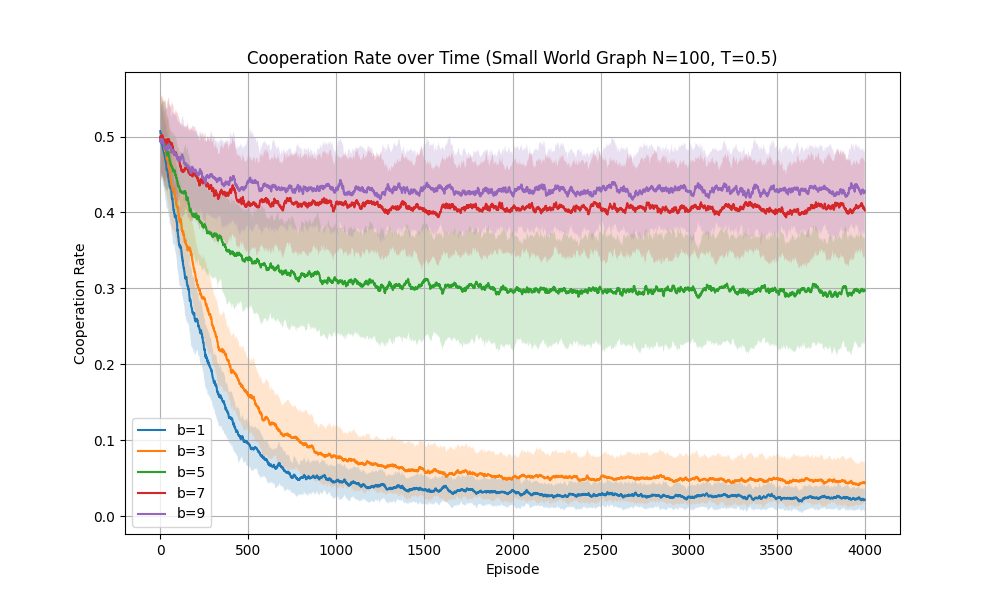
\includegraphics[width=0.9\textwidth]{../results/small_world_over_time_temp_0.5.png}
	\caption{Малый мир: динамика кооперации при $T=0.5, k_{anchors}=1$.}
	\label{fig:sw_t05}
\end{figure}

\begin{figure}[H]
	\centering
	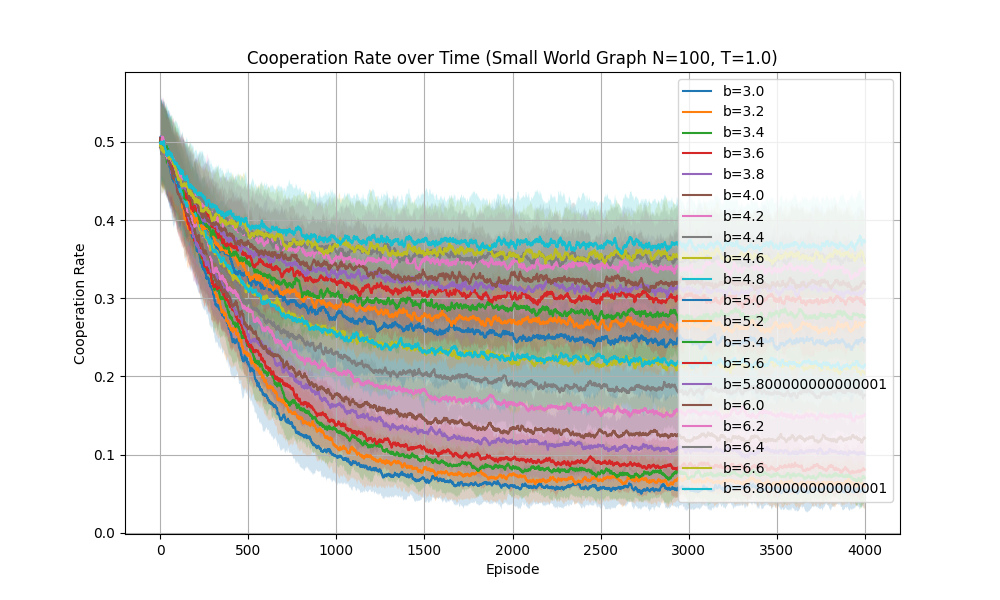
\includegraphics[width=0.9\textwidth]{../results/small_world_over_time_temp_1.0.png}
	\caption{Малый мир: динамика кооперации при $T=1.0, k_{anchors}=1$.}
	\label{fig:sw_t10}
\end{figure}

\begin{figure}[H]
	\centering
	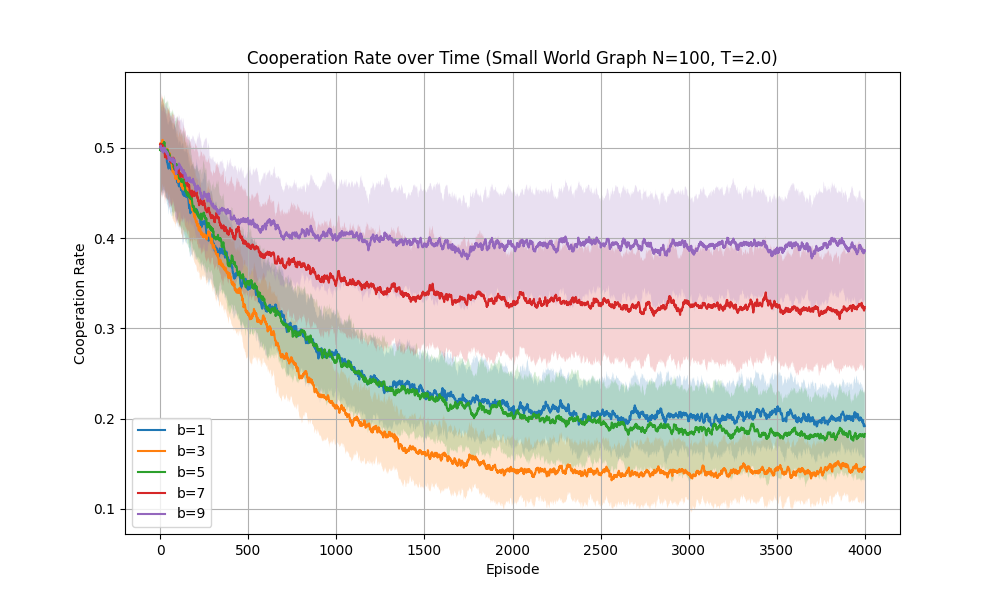
\includegraphics[width=0.9\textwidth]{../results/small_world_over_time_temp_2.0.png}
	\caption{Малый мир: динамика кооперации при $T=2.0, k_{anchors}=1$.}
	\label{fig:sw_t20}
\end{figure}

\begin{figure}[H]
	\centering
	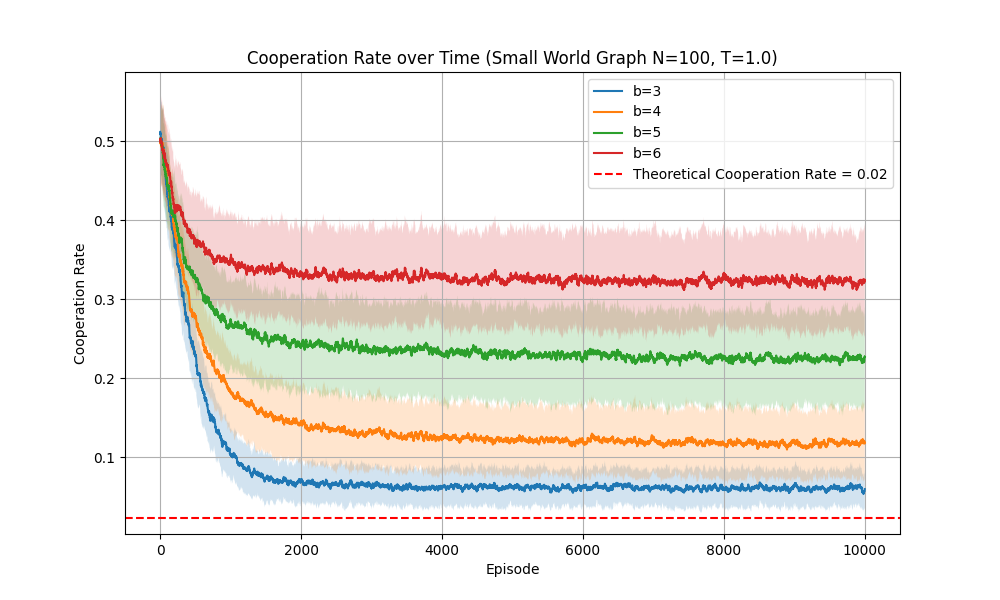
\includegraphics[width=0.9\textwidth]{../results/small_world_over_time_temp_1.0_many_exps.png}
	\caption{Малый мир: динамика кооперации (много запусков).}
	\label{fig:sw_many}
\end{figure}

\begin{figure}[H]
	\centering
	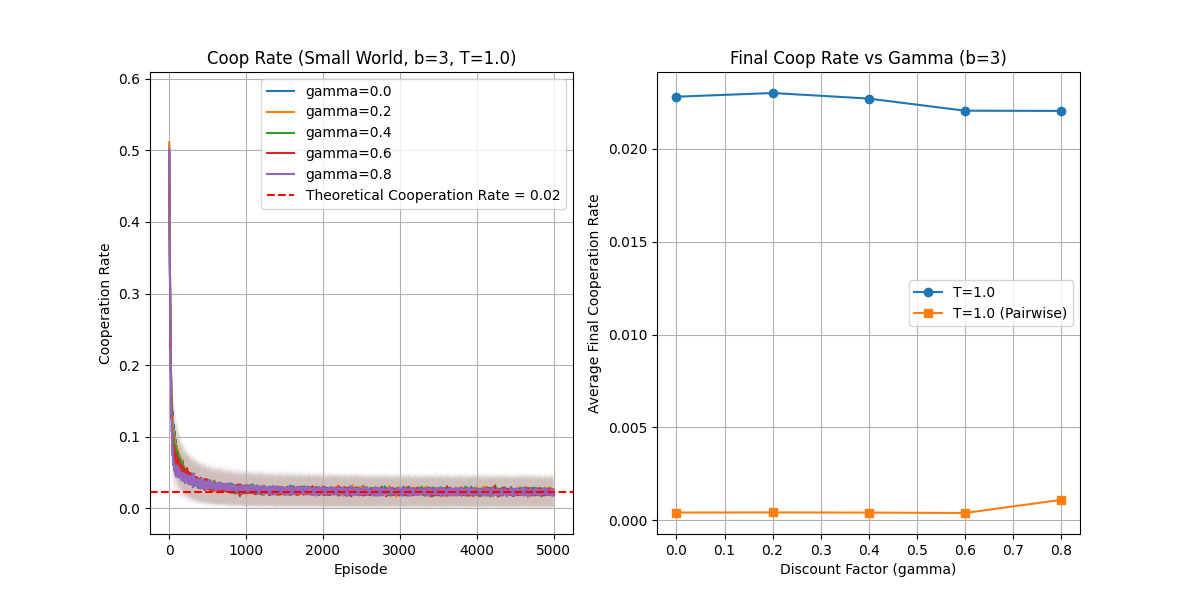
\includegraphics[width=0.8\textwidth]{../results/N_anchors/gamma_exp/small_world_vs_gamma_b_3_temp_1.0.png}
	\caption{Малый мир: финальная кооперация vs $\gamma$, $b=3$, $T=1.0$, $k_{anchors}=N$.}
	\label{fig:sw_gamma_b3}
\end{figure}

\begin{figure}[H]
	\centering
	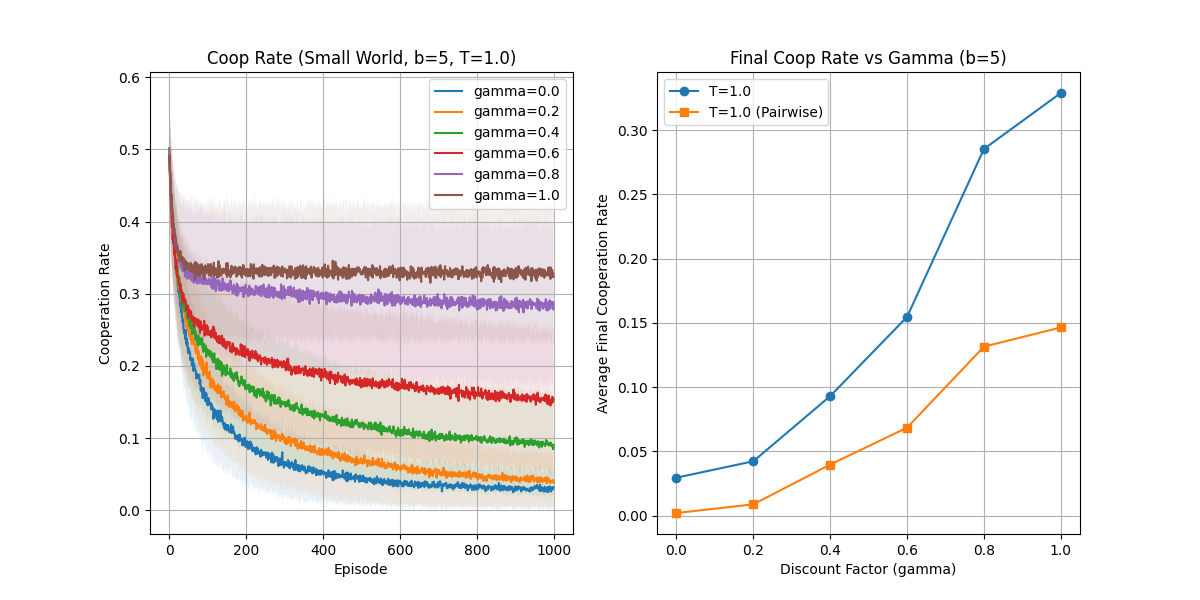
\includegraphics[width=0.8\textwidth]{../results/N_anchors/gamma_exp/small_world_vs_gamma_b_5_temp_1.0.png}
	\caption{Малый мир: финальная кооперация vs $\gamma$, $b=5$, $T=1.0$, $k_{anchors}=1$.}
	\label{fig:sw_gamma_b5}
\end{figure}

\section{Заключение}
Сформулирована модель обучения на графе с несколькими режимами игры,
реализованы Q-learning и SARSA с epsilon-greedy и Boltzmann политиками,
описаны четыре вида наград. Эксперименты на звезде и малом мире
показывают зависимость кооперации от $b$, $T$ и $\gamma$ и подтверждают,
что локальное (гранулярное) обновление может поддерживать кооперативные
кластеры. В дальнейшем планируется расширение на другие игры
и адаптивный выбор гранул.

\bibliographystyle{plain}
\bibliography{refs}

\end{document}